\section{Corrección del software}
La motivación para esta materia surge de la dificultad que presentan los programas concurrentes a la hora de intentar determinar su correctitud. En particular nos concentramos en los programas que responden a sistemas críticos (esto es, sistemas cuyas fallas pueden causar daños de gran importancia, incluyendo pérdidas de vidas humanas, catástrofes ecológicas, grandes pérdidas económicas, etc.) y reactivos (sistemas que responden a eventos de su entorno).

Más en detalle, los sistemas reactivos presentan características diferentes respecto a los transformacionales\footnote{Programas que toman una entrada del entorno, le aplican una transformación, y devuelven el resultado.}, las tres principales a nombrar son:
\begin{enumerate}
  \item No es posible determinar exactamente cuándo llegaran los eventos desde el entorno (son asincrónicos)
  \item No necesariamente computan resultados
  \item No suele requerirse que terminen (como es caso para los sistemas operativos, por ejemplo)
\end{enumerate}

Una primera estrategia ante este problema, podría ser la del testing. Sin embargo, esta estrategia presenta un problema claro: \textbf{el testing es capaz de detectar la presencia de errores en el código, pero no la ausencia de los mismos.} Además, como se verá más adelante, el espacio de estados\footnote{El espacio de estados de un sistema está formado por el conjunto de valores posibles para todas las variables del sistema, más los program counter de los procesos/hilos involucrados.} de estos sistemas crece exponencialmente con la cantidad de variables, por lo que pensar en poder lograr una cobertura suficiente con tests se vuelve irreal.

Este último punto nos permite descartar la segunda estrategia posible: la de la simulación. Dado que el espacio de estados crece de esta manera, pudiendo ser incluso infinito, la simulación puede no detectar problemas en el software.

La tercer estrategia posible es la de la verificación semi-automática de software. Esta presenta serias limitaciones: desde la teoría sabemos que, por ejemplo, decidir si un problema termina o no no es computable\footnote{\url{https://en.wikipedia.org/wiki/Halting_problem}}. Si imponemos algunas restricciones sobre las propiedades que queremos verificar, sin embargo, hay algunas tareas que pueden verificarse automáticamente\footnote{\url{https://en.wikipedia.org/wiki/Model_checking}}\footnote{\url{https://en.wikipedia.org/wiki/Static_program_analysis}}\footnote{\url{https://en.wikipedia.org/wiki/Dynamic_program_analysis}}.

Por los problemas expuestos anteriormente es que se propone el enfoque de modelar: utilizar modelos matemáticos con la expresividad suficiente para poder representar los sistemas que podamos llegar a querer implementar, y que permitan aplicar herramientas matemáticas para determinar las propiedades del sistema. Se adelanta que el modelo elegido en esta materia son las redes de Petri.

\section{El enfoque de modelar}
Se presentan dos modelos: las máquinas de estado finitas y las redes de Petri.

Si bien tienen menor expresividad, las primeras son más familiares para los programadores e ingenieros, tienen una semántica intuitiva, son fáciles de entender, y tienen una representación gráfica sencilla.

Es este punto, su representación gráfica, lo que las limita, ya que puede no ser práctico (o del todo posible) representar el espacio de estados de un sistema con ellas. Por esto se prefieren las redes de Petri.

\section{Programas concurrentes}
Los programas concurrentes están compuestos por componentes (procesos o hilos) que necesitan interactuar para, en general, llegar a un objetivo común.

Estos componentes concurrentes se ejecutan intercalando sus acciones atómicas\footnote{Atómicas se refiere a indivisible. Esto es, son operaciones que se ejecutan en su totalidad, o no se ejecutan, pero no pueden ser interrumpidas mientras lo están haciendo.} (esto se conoce como \textit{interleaving}). Esta intercalación queda en manos del scheduler, quien decide a qué hilo o proceso le toca tomar el CPU para ejecutarse. Estos schedulers son en general no deterministas, por lo que no se puede decidir el interleaving resultante de la ejecución de un programa, y un mismo par de procesos pueden tener ejecuciones diferentes.

La concurrencia puede presentarse en tres contextos:
\begin{enumerate}
  \item Múltiples aplicaciones, esto es, poder correr múltiples aplicaciones ``simultaneamente'' en un mismo core.
  \item Aplicaciones estructuradas, lo cual implica aplicar una estrategia \textit{divide \& conquer} en un mismo programa para implementar soluciones eficazmente.
  \item Estructura del sistema operativo, lo cual es simplemente aprovechar los beneficiones del contexto anterior, a nivel sistema.
\end{enumerate}

La misma comprende un gran número de cuestiones de diseño:
\begin{itemize}
  \item La comunicación entre procesos
  \item Compartición de y competencia por recursos
  \item Sincronización de la ejecución de varios procesos
  \item Asignación del tiempo a cada hilo o proceso
\end{itemize}

En general es muy difícil razonar sobre programas concurrentes debido a los diferentes interleavings que se pueden presentar: no siempre es claro cuáles son posibles de encontrar y cuales no a simple vista.

\subsection{Problemas comunes de los programas concurrentes}
Esta ejecución concurrente nos puede presentar ciertos problemas si no se toman las medidas adecuadas:
\begin{enumerate}
  \item  \textbf{Violación de propiedades universales}: por ejemplo, si tenemos una variable cuyos valores deben estar acotados, una mala programación concurrente puede llevar a que existan trazas de ejecución donde dichas cotas son sobrepasadas
  \item  \textbf{Starvation}: ocurre cuando uno o más procesos se quedan esperando indefinidamente un mensaje o evento. 
  \item  \textbf{Deadlock}: dos o más procesos se quedan esperando el avance del otro. Por ejemplo, tenemos dos procesos (A y B) que necesitan abrir los mismos dos archivos (input.txt y output.txt). El proceso A toma el archivo input.txt, y es interrumpido por el procesador, quien le da la CPU al proceso B. Este toma el archivo output.txt. Independientemente de si se siga ejecutando el proceso B o se le de la CPU al proceso A, ambos se van a bloquear esperando que se libere el archivo que les faltó tomar, lo cual nunca va a pasar.
  \item  \textbf{Uso no exclusivo de recursos compartidos}: es una generalización del primer problema, ya que puede que no exista una invariante, pero que el acceso incorrecto a una variable o un archivo afecten el funcionamiento del programa, o corrompan el valor almacenado.
  \item  \textbf{Livelock}: es similar al caso del deadlock, pero en esta situación los procesos al detectar que el otro recurso está tomado, liberan el suyo propio. Ambos realizan la misma acción, los dos recursos quedan disponibles, y los procesos vuelven a tomarlos y bloquearse mutuamente. La diferencia en este caso radica en que los procesos no están bloqueados, pero no están ``avanzando''.
\end{enumerate}

\section{Procesos}
Formalmente, un proceso es \textit{``una unidad de actividad que se caracteriza por la ejecución de una secuencia de intrucciones, un estado actual, y un conjunto de recursos del sistema asociados.''} Más prácticamente, es un programa (o parte de uno) en ejecución. En general se dividen programas en procesos para aprovechar los ``tiempos muetros.'' Esto es, si tengo que escribir algo a un archivo en el disco, puedo aprovechar el tiempo que se va a demorar dicha acción y seguir computando cosas en otro proceso, en vez de bloquear todo el programa hasta que la escritura esté lista.

Los servicios necesarios para la ejecución de y la comunicación\footnote{Se nombra la comunicación acá para remarcar el hecho de que toda comunicación entre procesos debe pasar por el kernel. Más adelante se verá que este es uno de los motivos por los cuales los hilos son ``más livianos.''} entre procesos quedan a cargo del sistema operativo. Al comienzo de la ejecución del programa, se inicia la ejecución de un proceso, el cual podrá a su vez generar \textit{procesos hijos}.

A su vez, estos pueden clasificarse según su sincronización desde sincronización fina (los procesos interactuan fuertemente, intercambiando mensajes cada un número reducido de operaciones), hasta procesos completamente independientes.

\subsection{Estados de los procesos}
El modelo de estados de los procesos depende del sistema operativo en cuestión (tanto del SO, como de la versión del mismo), pero en general, se puede resumir en 7 estados:
\begin{enumerate}
  \item \textbf{Creado}: ya existe en memoria, y las estructuras ya están listas, pero todavía no es reconocido por el sistema operativo.
  \item \textbf{En ejecución}: tiene el procesador actualmente
  \item \textbf{Esperando}: está listo para ejecutarse cuando le toque tiempo de procesador
  \item \textbf{Muerto}: por algún motivo terminó (o fue terminado), pero todavía no se liberan de la memoria sus estructuras
  \item \textbf{Bloqueado}: está a la espera de algún evento o señal de sinronización
  \item \textbf{Suspendido bloqueado}
  \item \textbf{Suspendido listo}
\end{enumerate}

Los últimos dos estados representan lo mismo que sus contrapartes no suspendidas, con la diferencia de que un proceso fue sacado de memoria y pasado al disco. Esto se hace generalmente para librerar memoria y evitar que el procesador quede oscioso.

\subsection{Control de procesos}
El control de los procesos por parte del sistema operativo se realiza mediante una estructura conocida como BCP (bloque de control de proceso) donde se tiene, entre otras cosas:
\begin{itemize}
  \item \textbf{Identificador} (PID)
  \item \textbf{Estado}
  \item \textbf{Contador de programa}
  \item \textbf{Valores de registros de la CPU} (para el cambio de contexto)
  \item \textbf{Espacio de direcciones de memoria}
  \item \textbf{Prioridad} (de ser utilizada por el algoritmo de planificación)
  \item \textbf{Lista de recursos y permisos asignados} (fds y sockets abiertos)
  \item \textbf{Estadísticas}
  \item \textbf{Datos del owner}
  \item \textbf{Signals pendientes}
\end{itemize}

\section{Hilos}
Los hilos surgen como una alternativa más ``liviana'' a los procesos. Funcionalmente se utilizan para lo mismo que los procesos, en el sentido de que son utilizados para dividir sistemas más complejos en subsistemas (ya sea para aprovechar tiempos muertos, paralelizar problemas, dividir y conquistar, etc.) 

A diferencia de los procesos, los hilos comparten recursos, como son: el espacio de memoria, los archivos abiertos, autenticación, etc. Esto hace que no sea necesario un cambio de contexto tan grande como con los procesos, por esto se dice que el switcheo entre hilos tiene menos overhead que entre procesos. Lo que es propio de cada hilo es el contador de programa, la pila de ejecución, y el estado de la CPU.

Mientras que en el caso de los procesos es el SO quien los gestiona, es este caso son gestionados por la JVM.

Por todo esto, si se tiene una aplicaión que debe implementarse como un conjunto de unidades de ejecición relacionadas, es más eficiente hacerlo con hilos que con procesos.

\subsection{Estados de los hilos}
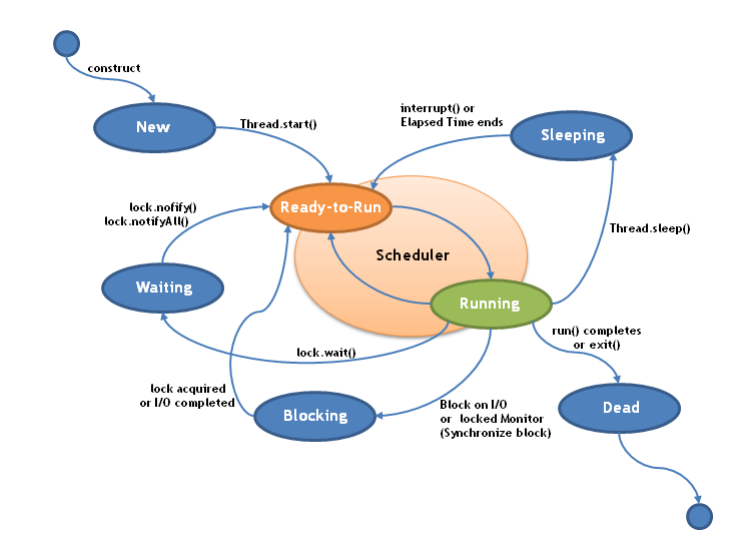
\includegraphics[width=\textwidth]{thread_statuses}
